\chapter{DESENVOLVIMENTO DO SISTEMA}
\label{chap:desenv}
Nesta seção serão explicitadas as características do manipulador JeRoTIMON, abordando os sistemas que o compõem em \textit{software} e em \textit{hardware}. Suas funcionalidades principais são abordadas e a conexão entre as mesmas é exibida. 

%------------------------------------------------------------------
\section{Descrição do sistema}
\label{sec:descsis}

JeRoTIMON é um manipulador desenvolvido para atender às demandas relacionadas ao reconhecimento de marcadores visuais e, a partir desta identificação, realizar o acionamento de um painel elétrico. Os pacotes que constituem este robô foram concebidos através do \textit{software} de simulação \textit{Gazebo}, da ferramenta de visualização \textit{Rviz} e do \textit{framework}\footnote{São conjuntos de aplicações dentro de um projeto que interagem entre si e com isso se alcança resultados como uma determinada função de um programa.} para planejamento de trajetória \textit{MoveIt}. O uso dessas ferramentas possibilita que uma grande variedade de atividades que venham a ser realizadas no mundo real tenham sido previamente testadas em ambiente computacional.

\subsection{Arquitetura geral}
\label{sub:arqg}

A Figura \ref{fig:arquitetura_geral} ilustra a estruturação do sistema e a relação entre \textit{software} e \textit{hardware}. As cores representam o sistema geral(salmão), sistema operacional(verde), \textit{framework}(roxo) e pacotes(azul).
\begin{figure}[H]
  \caption{Arquitetura geral do sistema.}
  \centering
  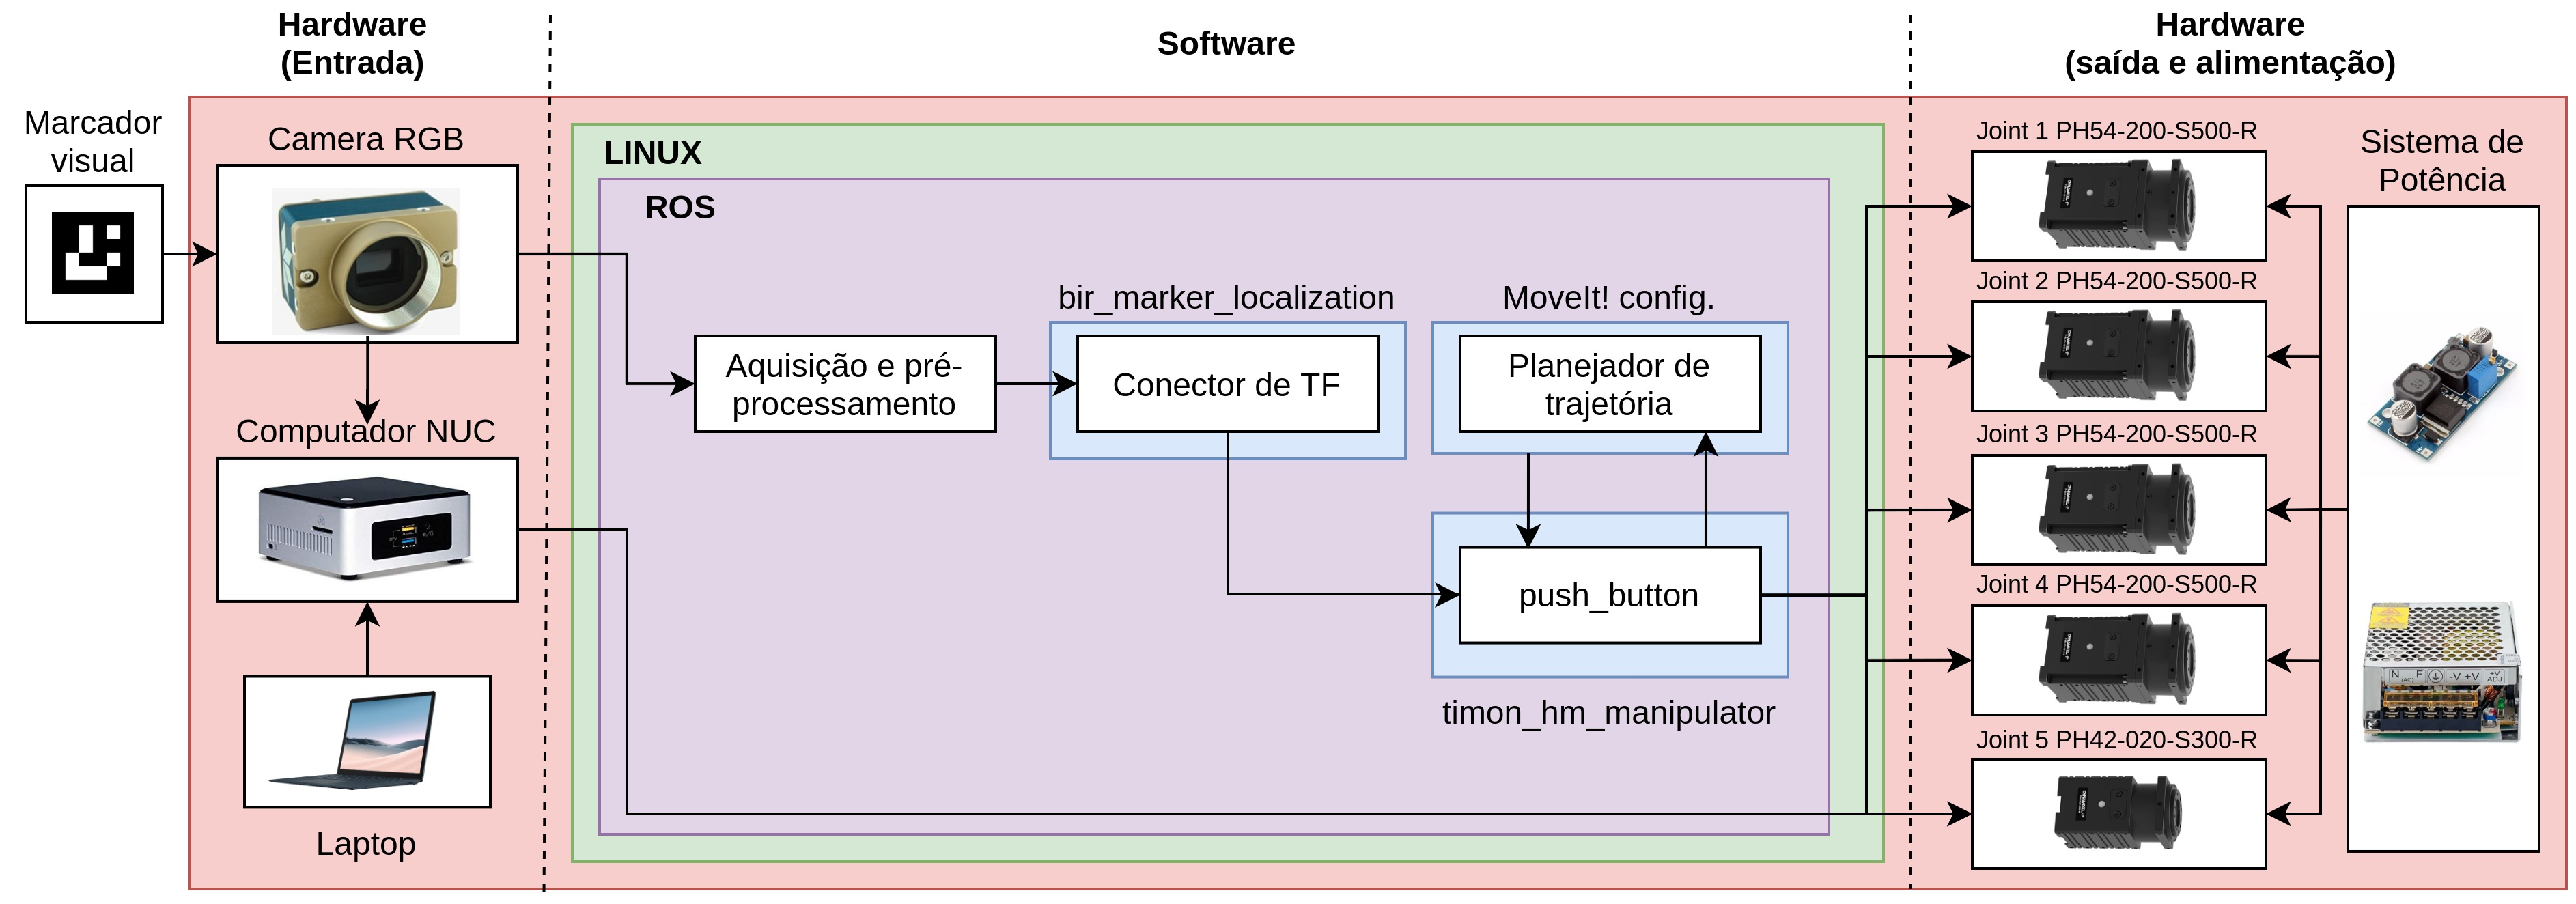
\includegraphics[width=16 cm]{images/arquitetura_geral.jpg}
    \label{fig:arquitetura_geral}
  \legend{Fonte: Autoria própria.}
\end{figure}

Um laptop, conectado via acesso remoto, dá início a aplicação no computador \textit{NUC}\footnote{Computador pequeno, completo e altamente eficiente energeticamente.} que possui instalado o software do protótipo.  Com o sistema iniciado, a câmera RGB é capaz de obter dados visuais do ambiente e enviá-los para o \textit{\acs{ROS}}.  Ao encontrar o marcador visual, o pacote \textit{bir\_marker\_localization} é capaz de unir as árvores de \textit{TF}\footnote{Pacote do \textit{\acs{ROS}} que permite verificar as relações entre os \textit{frames} na estrutura de árvore.} do painel elétrico e do manipulador, que antes encontravam-se desconectadas. Esta conexão, garante que sejam conhecidos os dados de posição ao nó \textit{push\_button} possibilitando o planejamento de trajetória para o ponto desejado. Com o caminho planejado, \textit{push\_button} pode enviar os comandos para cada junta do manipulador, onde encontram-se os motores \textit{Dynamixel} que são alimentadas pelo sistema de potência.

\subsection{Especificação técnica}
\label{sub:esptec}

Na Tabela \ref{tab:esp_table} estão elencadas as especificações técnicas do manipulador robótico JeRoTIMON. O numero de Graus de Liberdade foi definido baseado na capacidade de movimentação necessária para a realização dos desafios propostos. A carga útil, peso e o alcance máximo foram calculados com o auxilio do \textit{software} \textit{Onshape}, uma alternativa ao cálculo manual. A faixa de operação dos motores foi obtida segundo os limites de segurança observados, o que acrescenta proteção principalmente ao cabeamento do sistema. Informações a respeito de componentes como câmeras e motores seguem o seu padrão original de fabricação.

% \begin{table}[H]
%   \caption{Especificações técnicas do manipulador JeRoTIMON.}
%   \centering
%   \begin{tabular}{|c|c|}
%   \hline
%   \textbf{Item}                                                  & \textbf{JeRoTIMON}                                               \\ \hline
%   Graus de liberdade                                             & 5                                                               \\ \hline
%   \rowcolor[HTML]{EFEFEF} 
%   Carga útil                                                     & 1,94 kg                                                         \\ \hline
%   Alcance                                                        & \cellcolor[HTML]{FFFFFF}979 mm                                  \\ \hline
%   \rowcolor[HTML]{EFEFEF} 
%   Peso                                                           & 7,38 kg                                                         \\ \hline
%   Tensão de operação                                             & 24 V                                                            \\ \hline
%   \rowcolor[HTML]{EFEFEF} 
%   \cellcolor[HTML]{EFEFEF}                                       & Junta 1, Junta 2: 1.003.846 pulsos/rev                          \\ \cline{2-2}
%   \multirow{-2}{*}{\cellcolor[HTML]{EFEFEF}Resolução}            & Junta 3, Junta 4, Junta 5: 4096 pulsos/rev                       \\ \hline
%                                                                  & \cellcolor[HTML]{EFEFEF}Junta 1, Junta 2: H54-200-S500-R (200 W) \\ \cline{2-2}
%   \multirow{-2}{*}{Motores}                                      & Junta 3(2), Junta 4, Junta 5: MX-106 (65 W)                      \\ \hline
%   \rowcolor[HTML]{EFEFEF} 
%   \cellcolor[HTML]{EFEFEF}                                       & Junta 1: $ -90^\circ \sim 90^\circ $                      \\ \cline{2-2} 
%   \cellcolor[HTML]{EFEFEF}                                       & Junta 2: $ -90^\circ \sim 90^\circ $                      \\ \cline{2-2} 
%   \rowcolor[HTML]{EFEFEF} 
%   \cellcolor[HTML]{EFEFEF}                                       & Junta 3: $ -90^\circ \sim 135^\circ $                     \\ \cline{2-2} 
%   \cellcolor[HTML]{EFEFEF}                                       & Junta 4: $ -180^\circ \sim 180^\circ $                           \\ \cline{2-2} 
%   \rowcolor[HTML]{EFEFEF} 
%   \multirow{-5}{*}{\cellcolor[HTML]{EFEFEF}Faixa de operação}    & Junta 5: $ -90^\circ \sim 90^\circ $                      \\ \hline
%   Camera                                                         & Teledyne Genie Nano C2590                                             \\ \hline
%   \rowcolor[HTML]{EFEFEF} 
%   \cellcolor[HTML]{EFEFEF}                                       & Pose inicial: Codificador Absoluto                                        \\ \cline{2-2} 
%   \multirow{-2}{*}{\cellcolor[HTML]{EFEFEF}Tipo do sensor de posição} & Controle: Codificador Incremental                                    \\ \hline
%   Communicação                                                   & RS485                                                           \\ \hline
%   \rowcolor[HTML]{EFEFEF} 
%   Taxa de transmissão                                            & 1 Mbps                                                          \\ \hline
%   \end{tabular}
%   \legend{Fonte: Autoria própria.}
%   \label{tab:esp_table}
%   \end{table}



  \begin{table}[H]
    \caption{Especificações técnicas do manipulador JeRoTIMON.}
    \begin{tabular}{|c|c|}
    \hline
    \rowcolor[HTML]{EFEFEF} 
    \textbf{Item}                                              & \textbf{JeRoTIMON}                                             \\ \hline
    \textbf{Graus de liberdade}                                & 5                                                              \\ \hline
    \rowcolor[HTML]{EFEFEF} 
    \textbf{Carga útil}                                        & 2 {[}kg{]}                                                     \\ \hline
    \textbf{Alcance}                                           & 981 {[}mm{]}                                                   \\ \hline
    \rowcolor[HTML]{EFEFEF} 
    \textbf{Peso (sem base)}                                   & 6,4 {[}kg{]}                                                   \\ \hline
    \textbf{Peso (com base)}                                   & 10 {[}kg{]}                                                    \\ \hline
    \rowcolor[HTML]{EFEFEF} 
    \textbf{Tensão de operação}                                & 24 {[}V{]}                                                     \\ \hline
                                                               & Junta 1, Junta 2, Junta 3, Junta 4: 1,003,846 {[}pulsos/rev{]} \\ \cline{2-2} 
    \multirow{-2}{*}{\textbf{Resolução}}                       & Junta 5: 607,500 {[}pulsos/rev{]}                              \\ \hline
    \rowcolor[HTML]{EFEFEF} 
    \cellcolor[HTML]{EFEFEF}                                   & Junta 1, Junta 2, Junta 3: PH54-200-S500-R (200 W)             \\ \cline{2-2} 
    \rowcolor[HTML]{EFEFEF} 
    \cellcolor[HTML]{EFEFEF}                                   & Junta 4: PH54-100-S500-R (100W)                                \\ \cline{2-2} 
    \rowcolor[HTML]{EFEFEF} 
    \multirow{-3}{*}{\cellcolor[HTML]{EFEFEF}\textbf{Motores}} & Junta 5: PH42-020-S300-R (20 W)                                \\ \hline
                                                               & Junta 1: $ -45^\circ \sim 45^\circ $                           \\ \cline{2-2} 
                                                               & Junta 2: $ -90^\circ \sim 90^\circ$                            \\ \cline{2-2} 
                                                               & Junta 3: $ -43^\circ \sim 173^\circ $                          \\ \cline{2-2} 
                                                               & Junta 4: $ -90^\circ \sim 90^\circ $                           \\ \cline{2-2} 
    \multirow{-5}{*}{\textbf{Faixa de operação}}               & Junta 5: $ -90^\circ \sim 90^\circ $                           \\ \hline
    \rowcolor[HTML]{EFEFEF} 
    \textbf{Câmera}                                            & Teledyne Genie Nano C2590                                      \\ \hline
                                                               & Pose inicial: Codificador Absoluto                             \\ \cline{2-2} 
    \multirow{-2}{*}{\textbf{Tipo de sensor de posição}}       & Controle: Codificador Incremental                              \\ \hline
    \rowcolor[HTML]{EFEFEF} 
    \textbf{Comunicação}                                       & USB                                                            \\ \hline
    \textbf{Padrão elétrico}                                   & \cellcolor[HTML]{FFFFFF}RS485                                  \\ \hline
    \rowcolor[HTML]{EFEFEF} 
    \textbf{Taxa de transmissão}                               & 57,600 {[}bps{]}                                               \\ \hline
    \end{tabular}
    \legend{Fonte: Autoria própria.}
    \label{tab:esp_table}
    \end{table}




% \subsection{Características do manipulador}
% \label{sub:carac}
Para estabelecer uma relação entre o \textit{endeffector} e a base do manipulador é necessário descrever o seu sistema de coordenadas em relação ao sistema de coordenadas de origem. Para isto, é utilizada a notação de \textit{Denavit-Hartenger}(D-H). A partir da configuração D-H exibida na Figura \ref{fig:dh_config} foram retirados os parâmetros exibidos na tabela \ref{tab:dh}.


\begin{figure}[H]
    \caption{Configuração D-H do manipulador JeRoTIMON.}
    \centering
    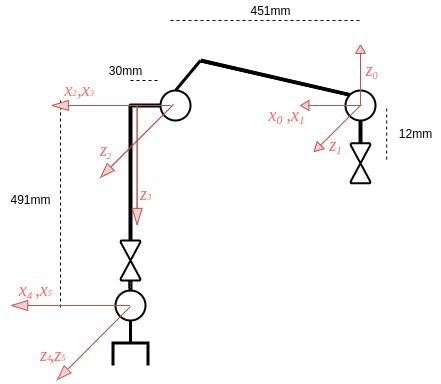
\includegraphics[scale=0.8]{images/dh_configuration.png}
    \legend{Fonte: Autoria própria.}
    \label{fig:dh_config}
\end{figure}

\begin{table}[H]
    \caption{Parâmetros D-H para o manipulador JeRoTIMON.}
    \centering
    \begin{adjustbox}{max width=\textwidth}
    \begin{tabular}{|c|c|c|c|c|}
    \hline
    \rowcolor[HTML]{EFEFEF} 
    Link & a (mm) & $\alpha(^\circ) $ & d (mm) & $\theta(^\circ)$ \\ \hline
    1 & 0   & $90$ & 12  & 0                     \\ \hline
    \rowcolor[HTML]{EFEFEF} 
    2 & 452 & 0         & 0   & $90 - \arctan(30/451)$ \\ \hline
    3 & 30  & $-90$  & 0   & $45 + \arctan(30/451)$ \\ \hline
    \rowcolor[HTML]{EFEFEF} 
    4 & 0   & $90$   & 491 & 0                     \\ \hline
    5 & 0   & 0         & 0   & 0                     \\ \hline
    \end{tabular}
    \end{adjustbox}
    \legend{Fonte: Autoria própria.}
    \label{tab:dh}
    \end{table}



\subsection{Ambiente de operação}
\label{sub:ambiente}

O ambiente físico para a realização do desafio, onde serão incluídos o manipulador e um painel elétrico, é uma mesa com 1.7 m de comprimento por 0.8 m de largura. É necessário então que verifique-se quais os pontos deste ambiente de trabalho que estão dentro da área de alcance (\textit{workspace})\footnote{É a área de alcance do manipulador, região na qual este consegue operar.} do manipulador.

A partir da tabela \ref{tab:dh} foi desenvolvido um código utilizando o software \textit{Matlab R2020a} capaz de gerar pontos que populem o \textit{workspace} do manipulador nas projeções dos planos X-Y, X-Z e Y-Z, conforme exibido nas figuras \ref{fig:workspace_xy}, \ref{fig:workspace_xz} e \ref{fig:workspace_yz}. A região em azul indica o alcance do robô e, a partir destas imagens, é possível observar que o manipulador possui restrições de operação devidas às limitações existentes em cada junta.


% \begin{figure}[H]
%     \caption{Simulação no Gazebo}
%     \centering
%     \includegraphics[scale=0.34]{images/desafio.png}
%     \legend{Fonte: Autoria própria.}
%     \label{fig:simulacao}
% \end{figure}


\begin{figure}[H]
    \caption{\textit{Workspace} do manipulador no plano X-Y.}
    \centering
    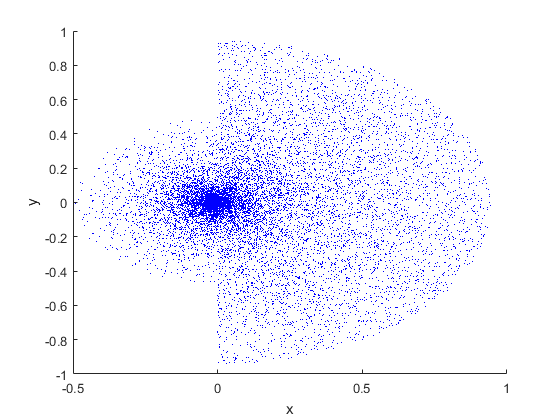
\includegraphics[scale=0.8]{images/workspace_xy.png}
    \legend{Fonte: Autoria própria.}
    \label{fig:workspace_xy}
\end{figure}



\begin{figure}[H]
    \caption{\textit{{Workspace}} do manipulador no plano  X-Z.}
    \centering
    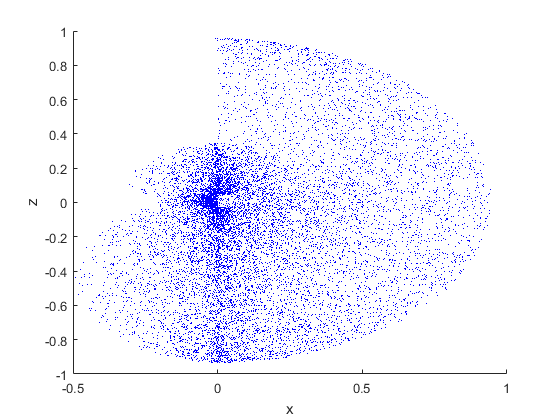
\includegraphics[scale=0.8]{images/workspace_xz.png}
    \legend{Fonte: Autoria própria.}
    \label{fig:workspace_xz}
\end{figure}


\begin{figure}[H]
    \caption{\textit{{Workspace}} do manipulador no plano  Y-Z.}
    \centering
    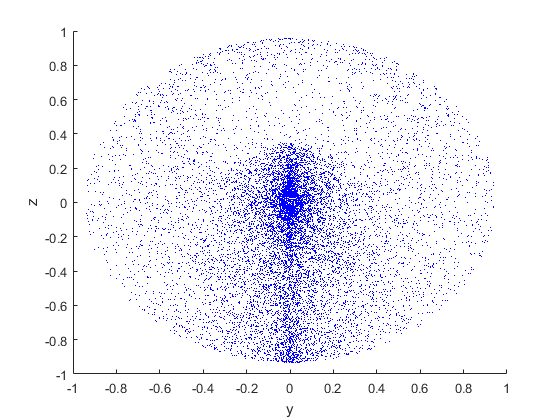
\includegraphics[scale=0.8]{images/workspace_yz.png}
    \legend{Fonte: Autoria própria.}
    \label{fig:workspace_yz}
\end{figure}

\subsection{Estrutura analítica do protótipo}
\label{sub:eap}

A estrutura analítica do protótipo mostrada na Figura \ref{fig:estrutura_analitica} exibe as relações sistemáticas entre as partes que compõem o manipulador. A estrutura hierárquica possui três níveis: o primeiro, referente ao sistema principal JeRoTIMON; o segundo, que é composto pelos sub-sistemas de potência, aquisição, processamento, estrutura e atuação; e o terceiro, composto pelos itens que fazem parte de cada um destes sub-sistemas. 

\begin{figure}[H]
  \caption{Estrutura analítica do protótipo.}
  \centering
  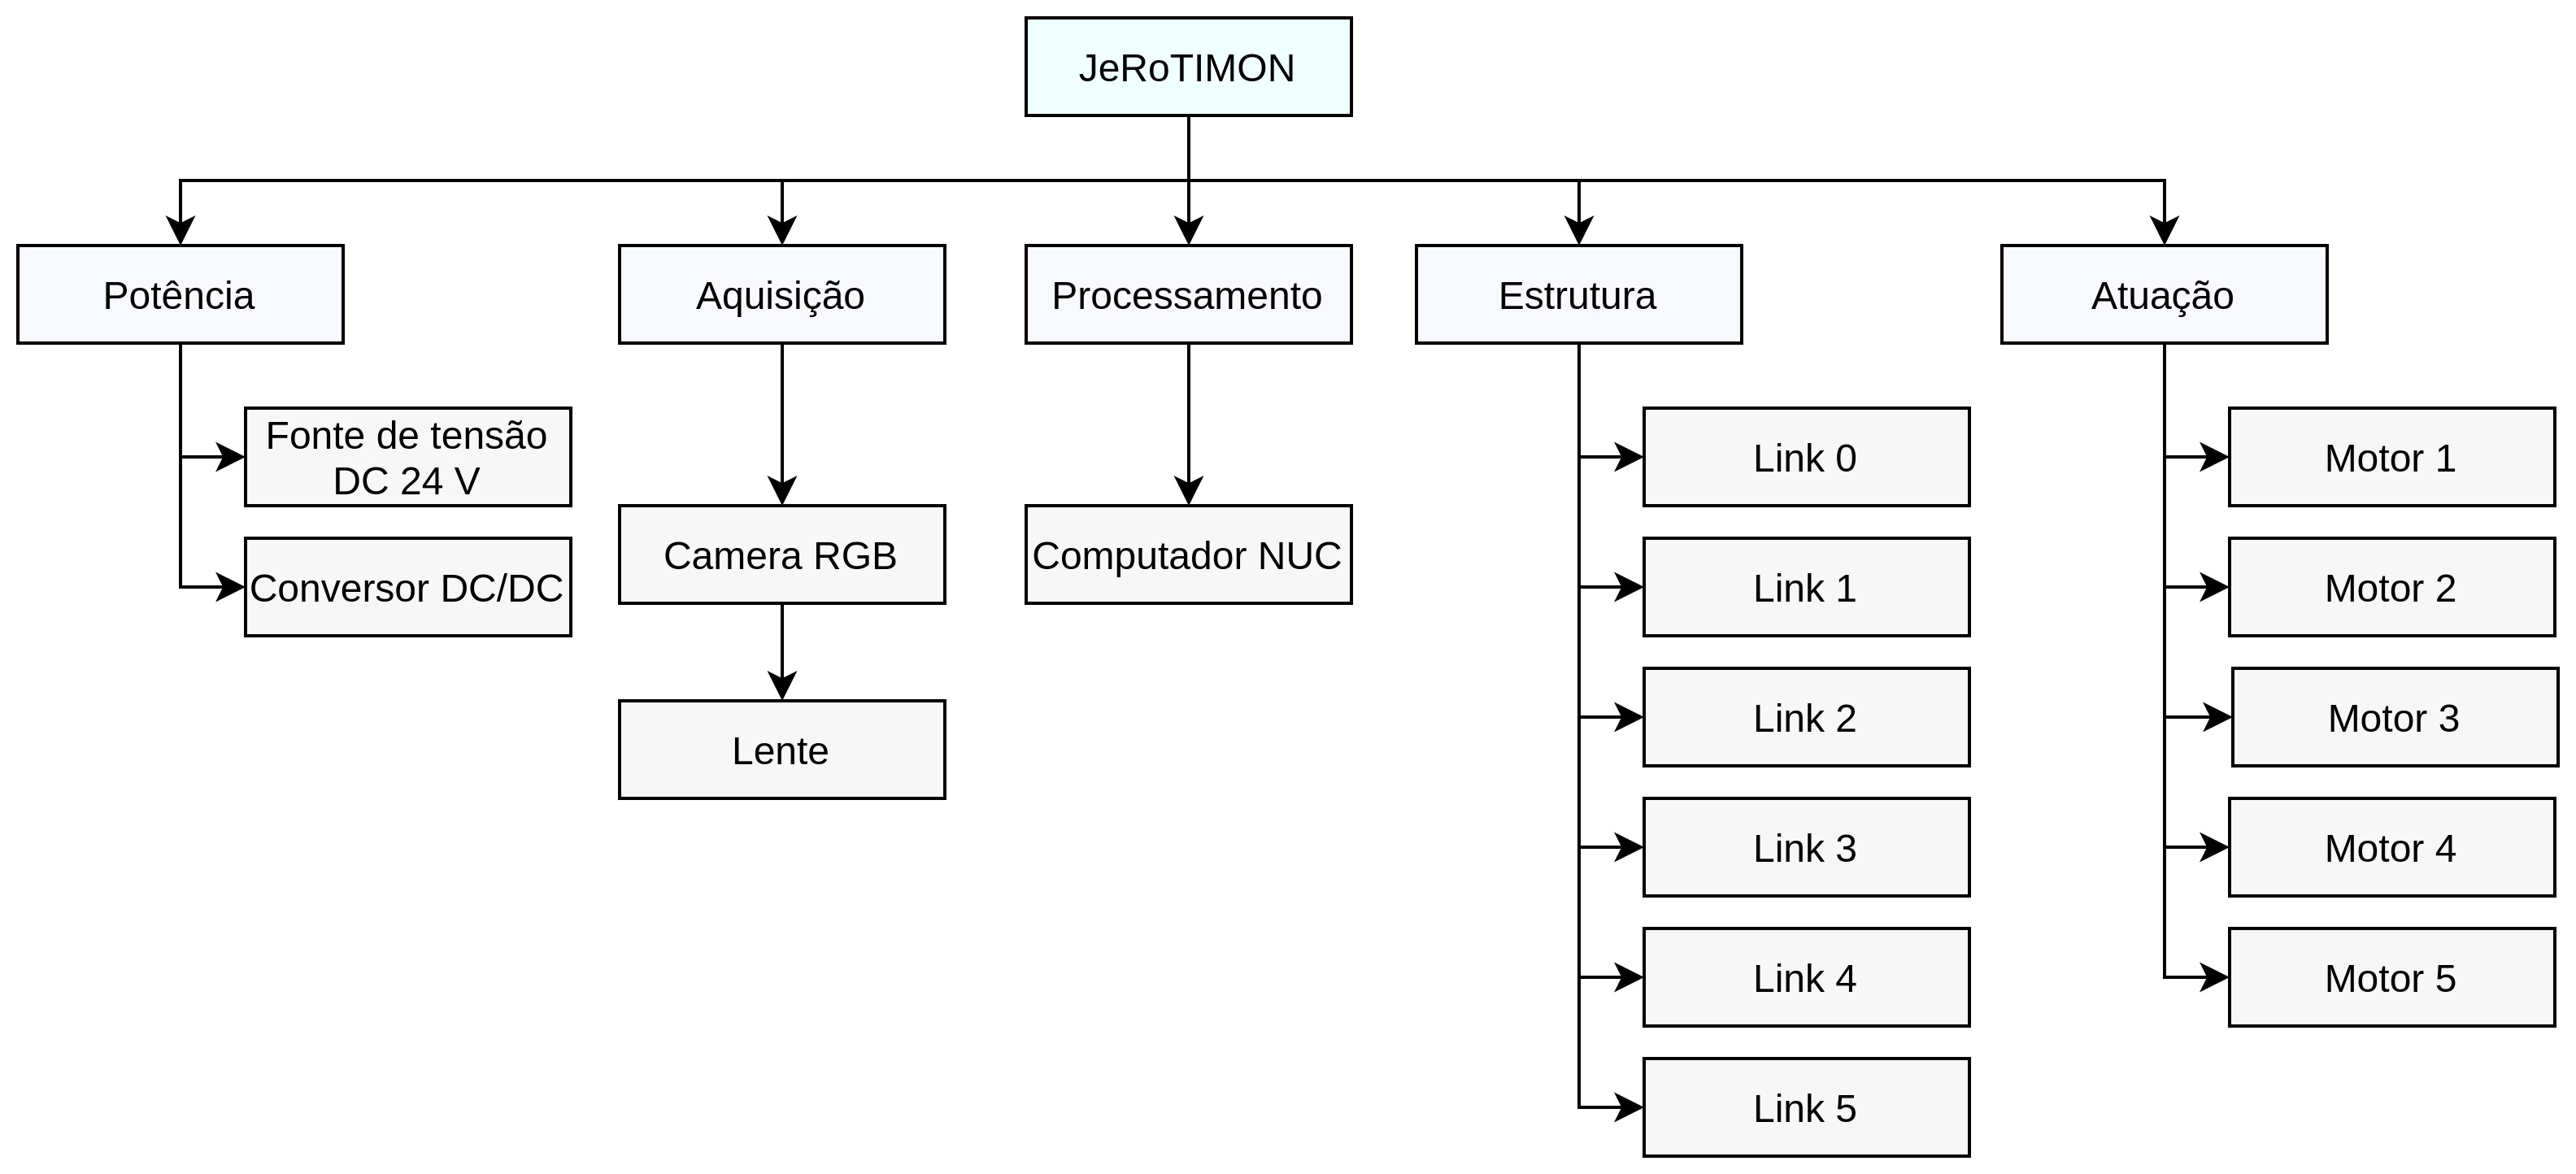
\includegraphics[width=16 cm]{images/estrutura_analitica.jpg}
  \legend{Fonte: Autoria própria.}
  \label{fig:estrutura_analitica}
\end{figure}


%------------------------------------------------------------------
\section{Especificação funcional} %na introdução da seção apresentar a conexão entre as funcionalidades
\label{sec:sota}
O manipulador descrito trabalha acionando os botões encontrados pelo sistema de aquisição. Seu software funciona baseado na troca de mensagens entre duas funcionalidades principais: Escaneamento e Planejamento/Execucção de trajetória. O Escaneamento corresponde à detecção de um marcador visual, que uma vez detectado, informa a posição no espaço de um painel elétrico que precisa ser acionado. O planejamento e execução de trajetória utiliza cálculos de cinemática direta e inversa para definir a trajetória de movimentação que permitirá ao manipulador realizar sua tarefa.


\subsection{Escaneamento}
\label{sub:funcA}

Uma câmera RGB \textit{Teledyne Genie Nano C2590} equipada com lente \textit{kowa LM8FC} foi acoplada ao manipulador JeRoTIMON. Através da mesma é realizada a detecção do marcador visual, utilizando a biblioteca \textit{ArUco} e o pacote \textit{Bir Marker Localization}, hospedado no site do Github no perfil do BIR - Brazilian Institute of Robotics \cite{birmarker}. 

\subsubsection{Descrição} 
\label{ssub:descA}
 
A Figura \ref{fig:flux_vis} exibe o fluxograma que descreve o funcionamento do sistema de escaneamento integrado ao manipulador. Após a captura  da imagem, a partir da câmera RGB, é feito um processamento dos dados obtidos afim de localização da \textit{tag} \textit{ArUco}, cujos tamanho e ID foram previamente estabelecidos. Caso o marcador seja encontrado, as árvores de \textit{TFs} do painel elétrico onde encontra-se o marcador, e do manipulador robótico são conectadas, possibilitando a localização no espaço da pose alvo. Os apêndices \ref{apend:tf1} e \ref{apend:tf2} exibem as árvores de \textit{TFs} antes e após a conexão realizada.

\begin{figure}[!ht]
  \caption{Fluxograma do sistema de escanamento.}
  \centering
  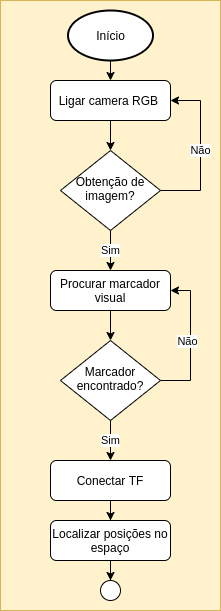
\includegraphics[scale=0.6]{images/fluxograma_sis_vis.png}
  \label{fig:flux_vis}
  \legend{Fonte: Autoria própria.}
\end{figure}


\subsubsection{Premissas necessárias}
\label{ssub:premA}

\begin{itemize}[itemsep=3pt,parsep=3pt]
  \item Conter um marcador visual anexado ao painel elétrico.
  \item A orientação dos elementos envolvidos no escaneamento, câmera RGB e marcador visual, devem ser definidos conforme estabelecido pelo pacote \textit{bir\_marker\_localization}.
  \item Não haver oclusão do marcador visual.
  \item Nível de iluminação do ambiente suficiente para a execução da detecção.
  \item O marcador visual deverá possuir tamanho adequado para detecção.
\end{itemize}

\subsubsection{Dependências}
\label{ssub:depA}

Para realizar a etapa de detecção é necessária a instalação do \textit{\acs{OpenCV}} versão 3.3.1, \textit{driver GigE-V Framework} e a inserção dos pacotes \textit{bir\_marker\_localization} e \textit{def\_cam\_teledyne\_nano} no \textit{workspace} do manipulador.

% \begin{lstlisting}[frame=single]
%   $ git clone git@github.com:Brazilian-Institute-of-Robotics/bir_marker_localization.git
% \end{lstlisting}



\subsubsection{Saídas}
\label{ssub:saidaA}

É fornecida ao sistema resposta por meio de uma sequência de mensagens publicadas no tópico \textit{/timon/camera/image\_raw}. Estes dados são analisados pelo detector \textit{ArUco}, possibilitando seu uso em um pacote desenvolvido na linguagem C++ que determina a posição do painel elétrico associado ao marcador visual. 



\subsection{Planejamento e Execução de Trajetória}
\label{sub:funcB}

As equações cinemáticas são a base que possibilitam a pesquisa do movimento dos manipuladores. A cinemática inversa provê um conjunto de valores para as juntas do manipulador com o intuito de alcançar uma determinada pose pré-estabelecida do seu \textit{endeffector}. Para resolver as equações da cinemática inversa do JeRoTIMON, optou-se por utilizar o plugin TRAC-IK, um método alternativo ao padrão da inversa Jacobiana utilizado pelo \textit{MoveIt}. Este método se adequa bem a manipuladores que possuam limitações em suas juntas, ao contrário de algoritmos baseados no teorema de Newton \cite{beeson2015trac}. Para o planejamento de trajetória foi utilizada a biblioteca \textit{\acs{OMPL}} , uma coleção de algoritmos de planejamento utilizada por padrão no \textit{MoveIt} \cite{sucan2012open}.

\subsubsection{Descrição} 
\label{ssub:descB}

A Figura \ref{fig:flux_pos} exibe o funcionamento do sistema de planejamento e execução de trajetória aplicado ao manipulador. A pose do painel elétrico, determinada a partir do que foi mostrado em \ref{sub:funcA}, é enviada como entrada para o \textit{MoveIt}. Caso seja possível, é realizado o planejamento de uma trajetória para cada uma das juntas do manipulador, a fim de movê-lo para a pose desejada. Esta trajetória é então enviada para os atuadores das juntas, que passam a executá-la. Após a realização da rotina para o pressionamento do painel elétrico, o manipulador retorna para sua posição inicial. Caso alguma condição impeça o planejamento de trajetória, como por exemplo o posicionamento do painel elétrico fora da área de trabalho do manipulador ou falhas nas soluções para as equações da cinemática inversa, uma mensagem de alerta é exibida e o robô realiza uma nova tentativa de planejamento.

\begin{figure}[H]
  \caption{Fluxograma do sistema de planejamento e execução de trajetória.}
  \centering
  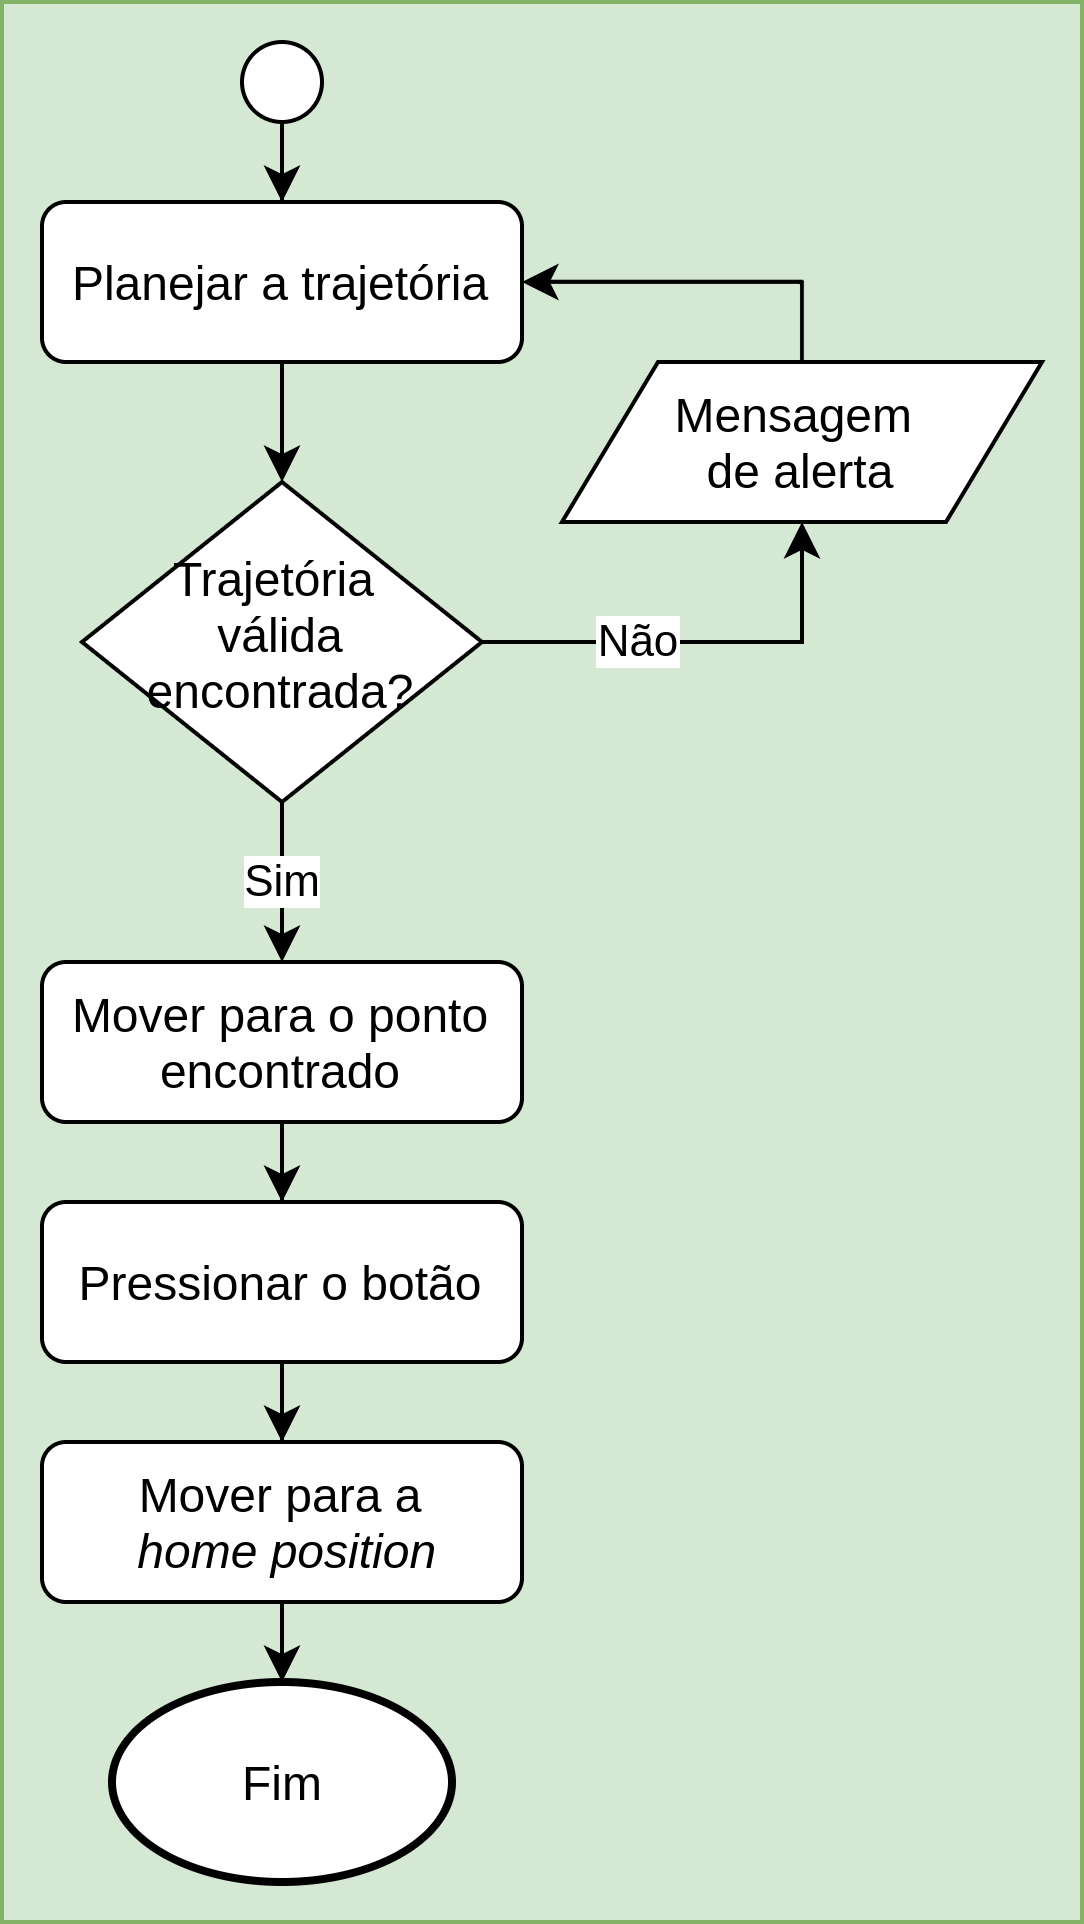
\includegraphics[scale=0.15]{images/fluxograma_plan_traj.png}
  \legend{Fonte: Autoria própria.}
  \label{fig:flux_pos}
\end{figure}
  

\subsubsection{Premissas necessárias}
\label{ssub:premB}
\begin{itemize}
    \item Viabilidade das soluções para cinemática inversa.
    \item Painel elétrico estar posicionado na área de trabalho do manipulador.
\end{itemize}

\subsubsection{Dependências}
\label{ssub:depB}
O sistema de movimentação é dependente da versão Melodic Morenia do \textit{framework} \textit{\acs{ROS}} e da plataforma \textit{MoveIt}. Além destes, uma lista de pacotes deve ser instalada previamente para o funcionamento correto do sistema:

    \begin{itemize}
      \item ros-melodic-ros-control
      \item ros-melodic-gazebo-ros-control
      \item ros-melodic-controller-manager
      \item ros-melodic-joint-trajectory-controller
      \item ros-melodic-joint-state-controller
      \item ros-melodic-position-controllers
      \item ros-melodic-trac-ik-kinematics-plugin
    \end{itemize}

\subsubsection{Saídas}
\label{ssub:saidaB}
As respostas fornecidas pelo sistema de planejamento e execução são publicadas nos  motores \textit{Dynamixel} integrados às juntas do manipulador. A trajetória gerada pelo \textit{MoveIt} pôde ser visualizada a partir do tópico \textit{/move\_group/display\_planned\_path} e é publicada nos motores a partir do tópico \textit{/timon\_arm\_controller/dynamixel\_state}.


%------------------------------------------------------------------
\section{Arquitetura de software}
\label{sec:arqs}
%introdução ao assunto apresentando a arquitetura
O robô JeRoTIMON foi desenvolvido para atuar em conjunto com o \textit{\acs{ROS}}, isto é, segue o propósito de conectar diferentes módulos, como câmeras, motores, sensores e códigos. A proposta é conectar um programa de visão capaz de conectar árvores de TF, através da identificação de marcadores visuais, com um sistema de movimentação que posiciona o manipulador para acionar o painel elétrico.

O apêndice \ref{apend:rqt} exibe o diagrama do \textit{software} do sistema, obtido via \textit{rqt\_graph}. Observa-se a comunicação entre o manipulador (\textit{/timon/robot\_state\_publisher}) e o painel elétrico (\textit{/box/box\_state\_publisher}) a partir da conexão das árvores de \textit{TFs} realizadas pelo \textit{/marker\_localization} que recebe e analisa os dados da câmera (\textit{/timon/camera\_image\_raw}). Pode-se verificar também que o nó \textit{/arm} comunica-se com o nó \textit{/move\_group} e com o nó \textit{/timon\_arm\_controller} a fim de enviar a trajetória planejada pelo \textit{MoveIt} para os motores \textit{dynamixel}.

%\subsection{Diagrama de componentes}
%\label{sub:diagcomp}


%\subsection{Matriz de rastreabilidade de testes}
%\label{sub:matrast}


%------------------------------------------------------------------
\section{Simulação do sistema}
\label{sec:simul}
A simulação do robô JeRoTIMON inserido em seu ambiente de trabalho foi realizada na plataforma \textit{Gazebo}. Para isto, realizou-se o desenvolvimento dos arquivos \textit{timon\_arm.urdf} e \textit{box.urdf}, modelos \textit{\acs{URDF}} que descrevem o robô e o painel elétrico a ser acionado. Foram levados em consideração características de massa, inércia e dimensão para cada componente destes modelos, para que houvesse maior fidelidade possível com o que representam fisicamente, de forma a garantir que os testes realizados possam ser validados em ambiente real. 

O pacote \textit{ros\_control} dispõe de uma lista de controladores disponíveis. Para JeRoTIMON, foram utilizados controladores do tipo \textit{position\_controllers/JointTrajectoryController}, e as transmissões para cada junta do manipulador foram definidas em seu modelo \textit{\acs{URDF}}.

Para simulação dâ câmera RGB, foi desenvolvido o arquivo \textit{camera.xacro}. O plugin padrão do \textit{Gazebo} foi utilizado, \textit{ligazebo\_ros\_camera.so} e as especificações da câmera RGB \textit{Teledyne Genie Nano C2590} foram levados em consideração, garantindo maior realismo à simulação. A figura \ref{fig:timon_gaz} exibe os modelos simulados do manipulador e do painel elétrico, enquanto a figura \ref{fig:camera_gaz} exibe imagem capturada pela câmera instalada no manipulador.


\begin{figure}[H]
  \caption{Modelos simulados do manipulador e do painel elétrico.}
  \centering
  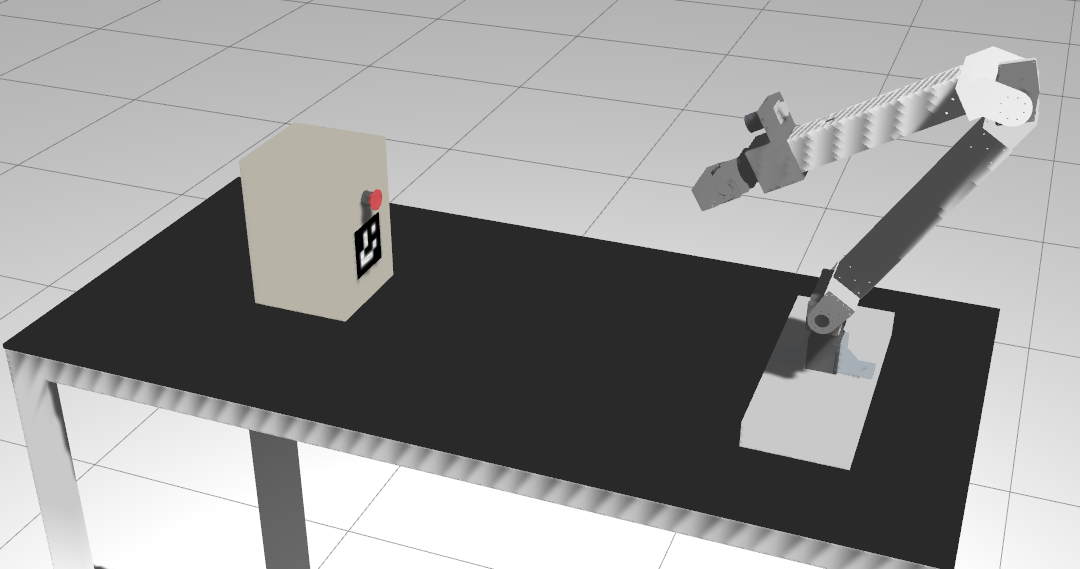
\includegraphics[scale=0.3]{images/timon.png}
  \legend{Fonte: Autoria própria.}
  \label{fig:timon_gaz}
\end{figure}


\begin{figure}[H]
  \caption{Imagem capturada pela câmera RGB.}
  \centering
  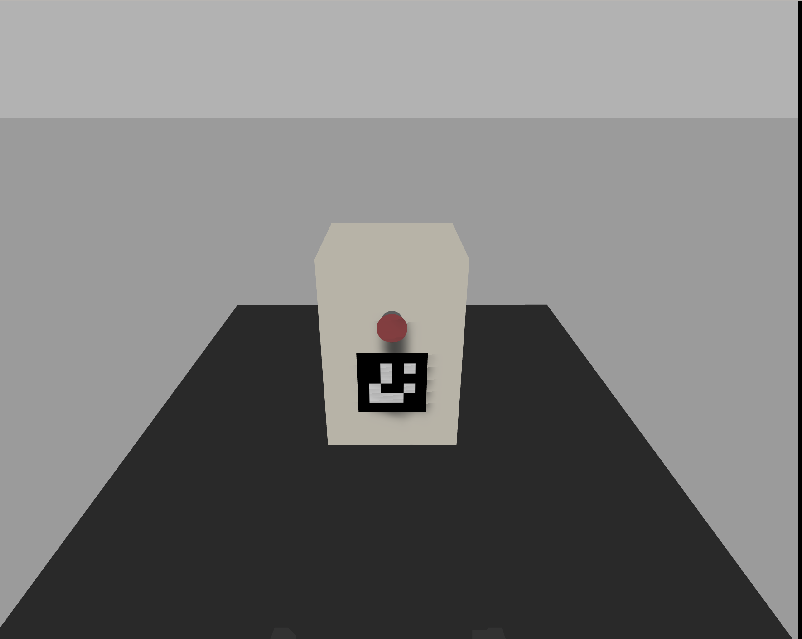
\includegraphics[scale=0.3]{images/camera.png}
  \legend{Fonte: Autoria própria.}
  \label{fig:camera_gaz}
\end{figure}

%\section{Integração}
%\label{sec:integra}





